\section{Rsnap}
\graphicspath{{content/7-solution/3-Rsnap/images/}}
Cette section traite de l'implémentation de la solution \gls{Rsnap} ainsi qu'une présentation de son utilisation.

\subsection{Implémentation}
Comme expliqués en section \ref{rails}, Rails possède une architecture Model-Vue-Controleur. Cette section va présenter l'application en se basant sur ce modèle d'architecture. La première partie explique le modèle, ensuite les contrôleurs sont abordés. Enfin, les vues sont présentées.

\subsubsection{Modèles}
Les concepts utiles pour développer l'application sont ceux présentés par les différents modèles dans la figure \ref{fig:models}.

\begin{figure}
 \begin{center}
   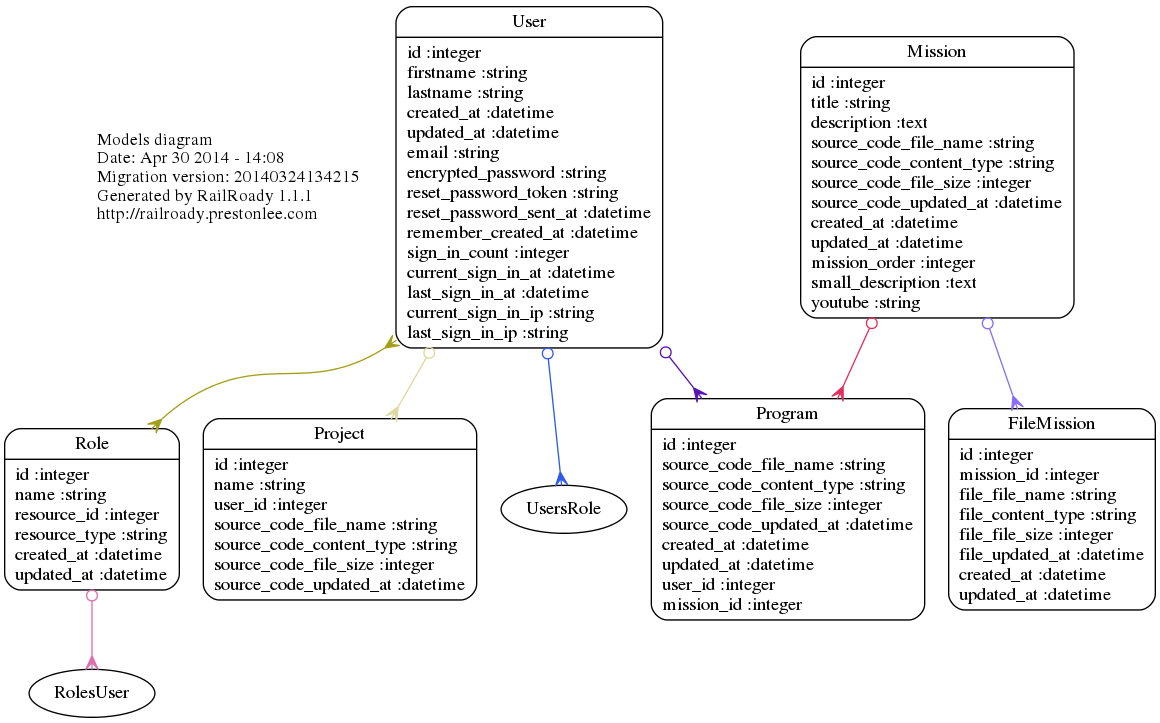
\includegraphics[width=\textwidth]{models_complete}
   \caption{Modèles de Rsnap}
   \label{fig:models}
 \end{center}
\end{figure}

\paragraph{\texttt{User}} Ce modèle contient les informations nécessaires pour identifier les utilisateurs (\texttt{firstname}, \texttt{email} \ldots) et pour les authentifier (\texttt{encrypted\_password}, \texttt{current\_sign\_in\_ip}, \ldots). Les utilisateurs peuvent posséder plusieurs rôles, programmes et projets.

\paragraph{\texttt{Role}} Les rôles permettent de donner des attributs aux utilisateurs. Ce modèle a été généré automatiquement par Rolify \ref{rolify}. Dans le cas de \gls{Rsnap}, deux types d'utilisateurs ont été créés : \texttt{admin} et \texttt{teacher}. Ces deux rôles sont globaux et ne sont donc pas rattachés à une ressource spécifique.

Les rôles sont utiles en conjonction avec les autorités \ref{authority} pour donner des droits supplémentaires à ces types d'utilisateurs.

\paragraph{\texttt{Mission}} Les missions représentent tout ce qui est nécessaire pour avoir un exercice. Une mission comporte donc un titre, une description avec des images et une vidéo pour expliquer à l'étudiant ce qu'il devra faire. De plus, elle comporte le code source initial de l'exercice. Généralement, celui-ci contient le squelette initial du programme pour l'étudiant et les tests pour vérifier le programme.

\paragraph{\texttt{FileMission}} Les fichiers liés à une mission sont les différentes images qui composent la description.

\paragraph{\texttt{Program}} Les programmes contiennent la solution d'un étudiant pour une mission. Ils contiennent uniquement le code source de l'étudiant.

\paragraph{\texttt{Project}} Les projets sont identiques aux programmes, mais ne sont pas liés à une mission. Ils contiennent donc le nom du projet en plus du code source.

\paragraph{Exemple} \texttt{Program} est un bon exemple de modèle Rails (code source \ref{lst:model-program}). Seules les fonctionnalités qu’Active Record \ref{active-record} ne sait pas déduire de lui-même sont présentes. Le modèle contient donc uniquement :
\begin{itemize}
  \item le nom des modèles avec qui il est associé et la cardinalité de la relation (\lstinline[language=Rails]{belongs_to} ligne 5-6) ;
  \item la validation de certains attributs pour qu'ils respectent certaines contraintes (\lstinline[language=Rails]{validates} ligne 13-15) ;
  \item des méthodes de classes pour simplifier les requêtes au modèle (\lstinline[language=Rails]{scope},  \lstinline[language=Rails]{self.*} ligne 17-23).
\end{itemize}

Comme c'est visible pour les \lstinline[language=Rails]{scope} à la ligne 17-19, Active Record permet de faire des requêtes SQL directement en Ruby.
\begin{figure}
\lstinputlisting[language=Rails, firstline=21, caption={Modèle \texttt{Program}}, label=lst:model-program]{content/7-solution/3-Rsnap/listings/program.rb}
\end{figure}

\subsubsection{Contrôleurs}
Les contrôleurs donnent accès à différentes ressources. La figure \ref{fig:controllers} montre la liste des contrôleurs implémentés pour cette application. La majorité de ceux-ci se rapporte directement à un modèle spécifique. Il existe néanmoins certaines ressources différentes telles que :
\begin{itemize}
  \item les pages statiques (\texttt{HomeController}) ;
  \item l'ordonnancement des missions (\texttt{SortMissionsController}) ;
  \item la création d'un programme depuis une mission (\texttt{InitializationMissionController}) ;
  \item les ressources utiles à l'affichage de Snap! (\texttt{SnapAssetsController}).
\end{itemize}

\begin{figure}
 \begin{center}
   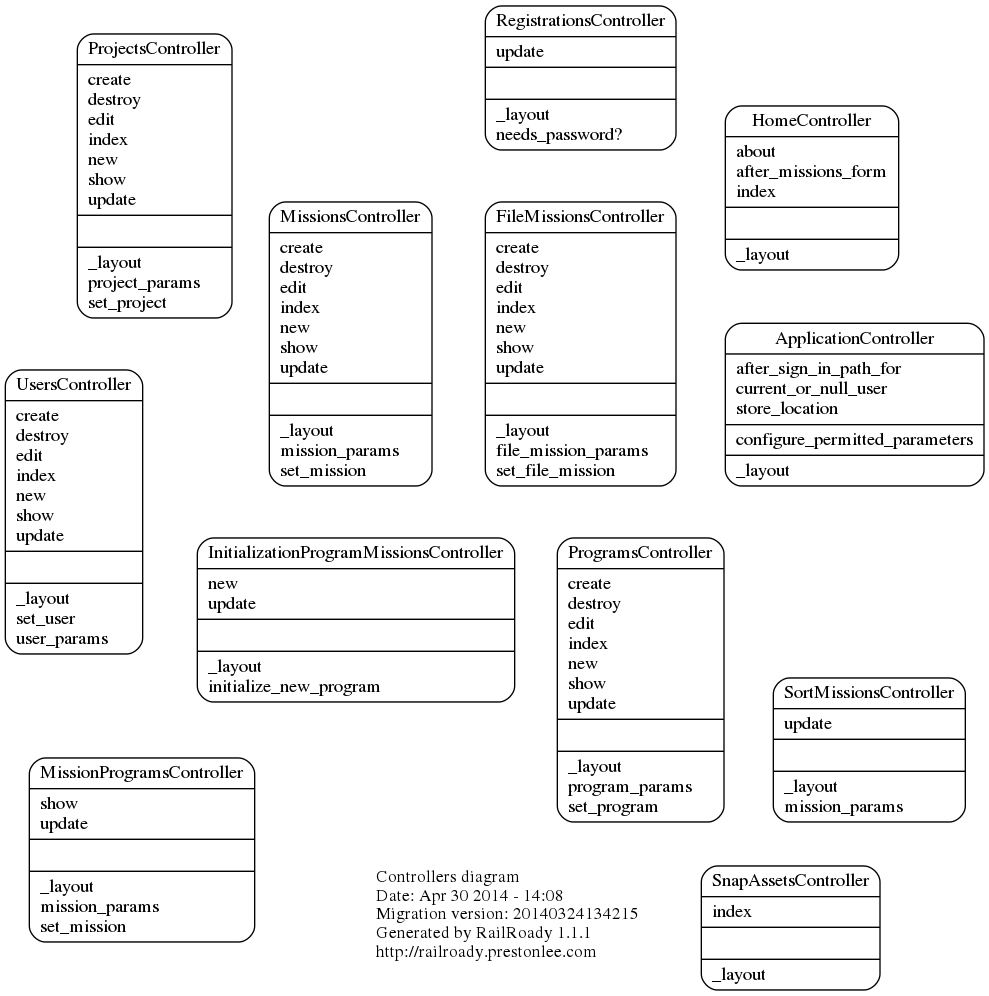
\includegraphics[width=\textwidth]{controllers_complete}
   \caption{Controlleurs de Rsnap}
   \label{fig:controllers}
 \end{center}
\end{figure}

Comme il est expliqué dans la section \ref{controleur}, les méthodes accessibles sont définies dans \texttt{routes.rb}. Les contrôleurs ont tous des ressources REST excepté \texttt{HomeController}. Ceci est visible dans \texttt{routes.rb} ou en regardant les fonctions publiques disponibles dans les contrôleurs sur la figure \ref{fig:controllers}.

\paragraph{Exemple}
L'extrait du contrôleur \texttt{MissionsController} \ref{lst:controller-mission} montre l'usage classique d'un contrôleur.

\begin{figure}
\lstinputlisting[language=Rails, linerange={1-5,10-34,52-62}, caption={Extrait du controlleur \texttt{MissionsController}}, label=lst:controller-mission]{content/7-solution/3-Rsnap/listings/missions_controller.rb} %TODO vérifier les ranges des lignes
\end{figure}

Grâce à la méta-programmation, \lstinline[language=Rails]{authorize_actions_for Mission} permet de rajouter, sur toutes les méthodes REST, des vérifications de ce que peut réaliser ou pas l'utilisateur courant. Ces vérifications sont injectées dans les autorités \ref{autority}. De plus, la méthode \lstinline[language=Rails]{before_filter} donne la possibilité de réaliser une action supplémentaire avant chaque appel de fonction. Dans cet exemple, il faut que l'utilisateur soit authentifié pour que l'application puisse ensuite vérifier ses droits. Ceci à l'exception des actions \texttt{show} et \texttt{index} qui peuvent être publiques.

Dans une méthode public d'un contrôleur plusieurs actions sont à implémenter :
\begin{enumerate}
  \item traiter, si nécessaire, les paramètres fournis. Ceux-ci se trouvent dans \lstinline[language=Rails]{params} ;
  \item Assigner les variables d'instance dont la vue a besoin pour s'afficher correctement ;
  \item Exécuter le rendu de la page. Cette étape est facultative si la vue a le même nom que la méthode.
\end{enumerate}

\subsubsection{Vue}
\label{vues}
Les vues sont écrites en haml \ref{haml}.

L'exemple de code \ref{lst:vue-user-index} avec \ref{lst:vue-user-partial} montre comment la vue servant à lister tous les utilisateurs est représentée (figure \ref{fig:vue-users}).

\begin{figure}
\lstinputlisting[language=haml, caption={Vue \texttt{index} des utilisateurs}, label=lst:vue-user-index]{content/7-solution/3-Rsnap/listings/index.html.haml}
\end{figure}

Le code source \ref{lst:vue-user-index} montre comment sont utilisées les variables d'instance créées par le contrôleur. Par exemple, la variable \texttt{@title} sert de titre 1.

\begin{figure}
\lstinputlisting[language=haml, caption={Vue d'une ligne \texttt{\_user} représentant un utilisateur}, label=lst:vue-user-partial]{content/7-solution/3-Rsnap/listings/_user.html.haml}
\end{figure}
De plus, Rails permet de faire le rendu d'un autre fichier de manière élégante. La ligne 14 du code source \ref{lst:vue-user-index} exécute le rendu sur tous les éléments de la collection \texttt{users} grâce au fichier \ref{lst:vue-user-partial}

Les connaisseurs de Bootstrap \ref{bootstrap} auront reconnu l'usage intensif des classes de style qu'il propose. L'adaptativité de cet outil est visible sur la capture d'écran \ref{fig:vue-users} : le menu supérieur a été réduit, car la taille de l'écran était trop petite pour accueillir le menu en entier.

\begin{figure}
  \begin{center}
    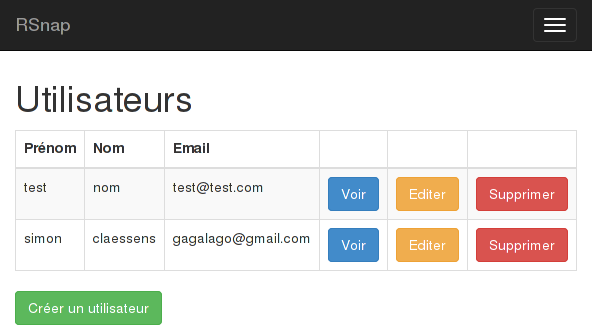
\includegraphics[width=.8\textwidth]{users}
    \caption{Affichage de la vue présentée par le code source \ref{lst:vue-user-index} et \ref{lst:vue-user-partial}}
    \label{fig:vue-users}
  \end{center}
\end{figure}

\subsection{Utilisation}
Pour utiliser la plateforme, il faut d'abord s'enregistrer. Ensuite, suivant le profil, différentes actions sont possibles. L'utilisateur normal peut uniquement résoudre les missions dans l'ordre proposé par les professeurs. Les professeurs peuvent aussi créer des missions. Cette section présente l'utilisation de la plateforme.
%TODO screenshot en annexe

\paragraph{Professeur}
Afin de réaliser un cours de programmation, un professeur doit pouvoir faire les actions suivantes :
\subparagraph{Créer des missions} Pour créer une nouvelle mission (figure \ref{fig:mission-create}), le professeur doit se rendre sur la page qui liste toutes les missions. Ensuite, il clique sur le bouton en bas de page "Nouvelle mission". Sur la page suivante, il donne les informations sur la mission : titre, description, explication de la mission, vidéo d'explication \ldots Il lui reste à créer la mission proprement dite. Lorsque le professeur clique sur le bouton "Créer une mission", il est redirigé vers l'interface de Snap!. Il peut alors créer tout ce qui est nécessaire à la réalisation et au test de la mission. Avant de sauver, il ne doit pas oublier de cacher les blocs et les scripts qui ne doivent pas être visibles par les étudiants.
\begin{figure}
  \begin{center}
    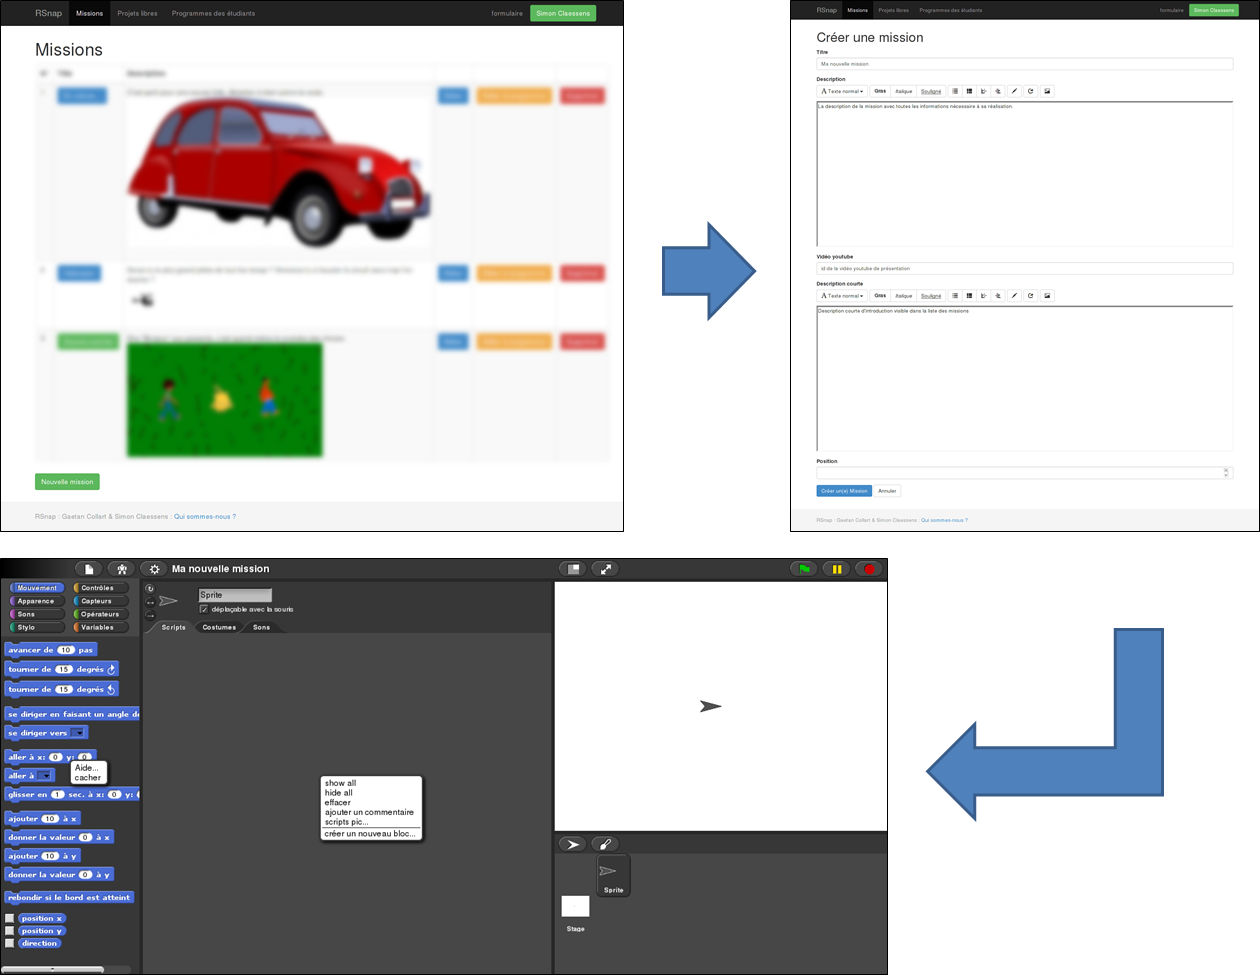
\includegraphics[width=.9\textwidth]{mission-create}
    \caption{Création d'une mission}
    \label{fig:mission-create}
  \end{center}
\end{figure}

\subparagraph{Ordonner les missions} Pour ordonner les missions (figure \ref{fig:mission-order}) dans un ordre pédagogique, il suffit de les glisser dans la liste.
\begin{figure}
  \begin{center}
    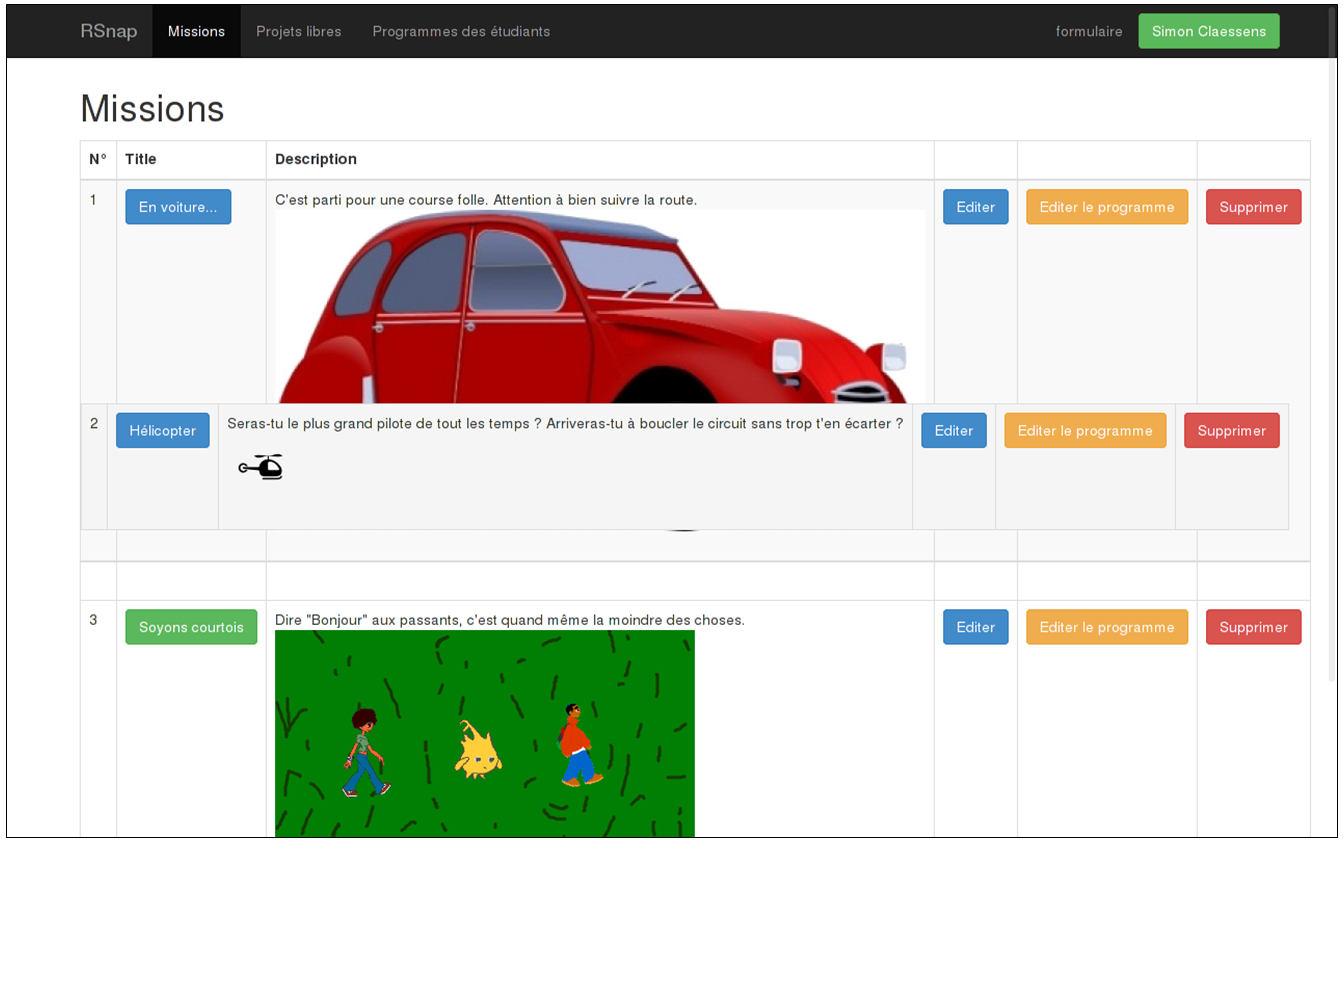
\includegraphics[width=.9\textwidth]{mission-order}
    \caption{Ordonner les missions}
    \label{fig:mission-order}
  \end{center}
\end{figure}

\subparagraph{Corriger les soumissions des étudiants} Pour corriger les soumissions de ses étudiants (figure \ref{fig:program-correction}), le professeur se rend sur la page des programmes. Il y sélectionne le programme qu'il désire corriger et qui s'ouvre dans l'interface Snap!. Le professeur peut alors rajouter des commentaires.
\begin{figure}
  \begin{center}
    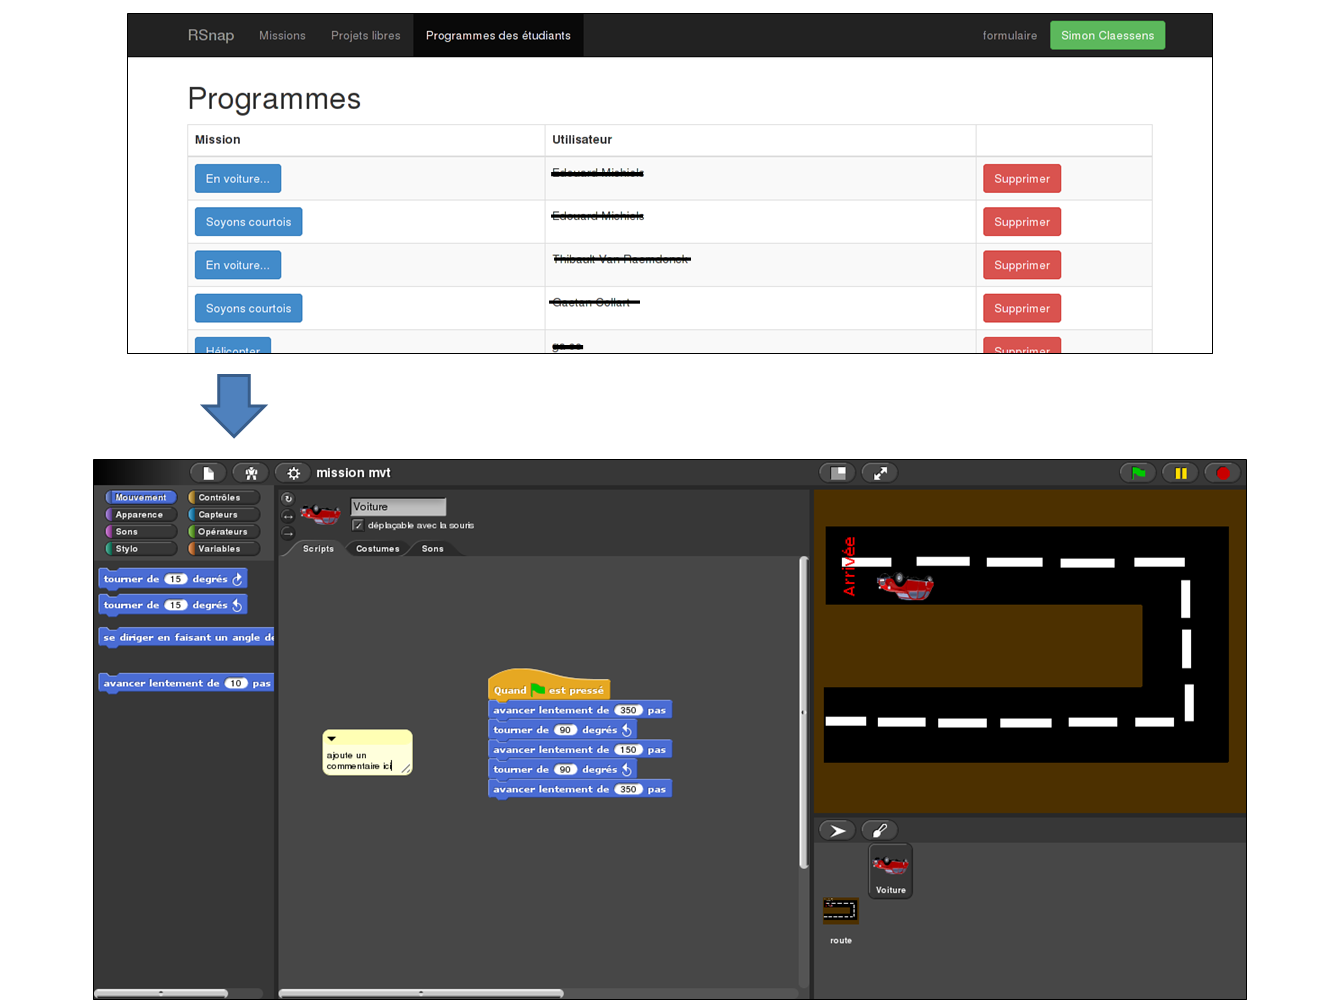
\includegraphics[width=.9\textwidth]{program-correction}
    \caption{Correction d'un programme}
    \label{fig:program-correction}
  \end{center}
\end{figure}

\paragraph{Étudiant}
Un étudiant doit pouvoir réaliser les opérations suivantes :
\subparagraph{Réaliser une mission} L'étudiant réalise une mission (figure \ref{fig:program-creation}) en cliquant sur le nom de la mission.

Deux possibilités s'offrent à lui. Soit le bouton est bleu, ce qui signifie que la mission a déjà été commencée. L'étudiant la reprend là où elle s'était arrêtée. Soit, le bouton est vert et dans ce cas, une nouvelle mission commence.

Dans les deux cas, l'étudiant se retrouve sur l'interface de Snap!.
\begin{figure}
  \begin{center}
    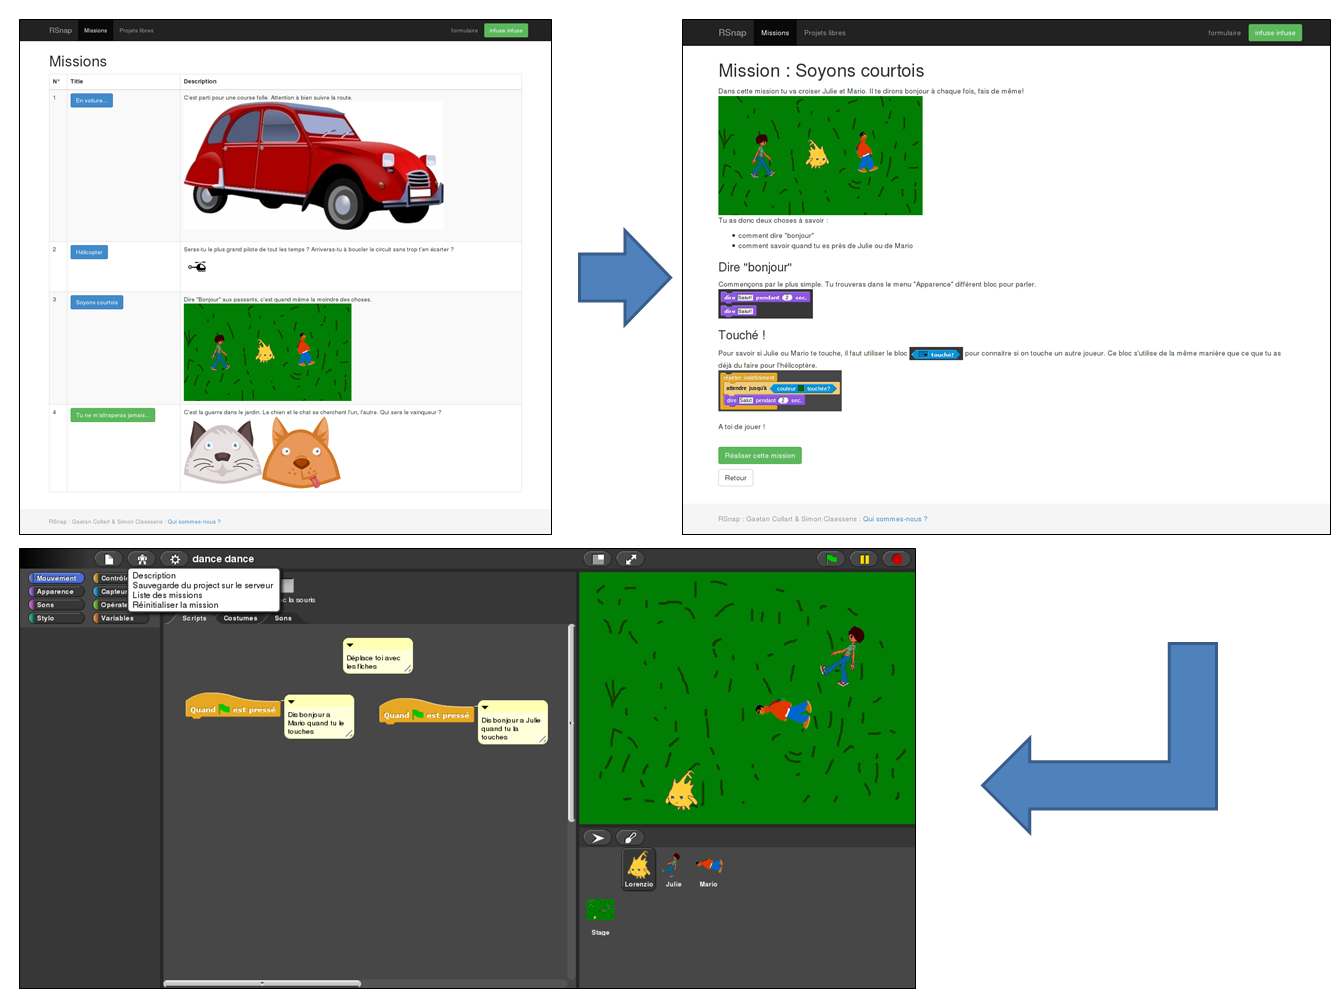
\includegraphics[width=.9\textwidth]{program-creation}
    \caption{Réalisation d'une mission}
    \label{fig:program-creation}
  \end{center}
\end{figure}

\subparagraph{Réaliser un projet libre} Si l'étudiant a envie de créer quelque chose (figure \ref{fig:project}), il va dans le menu "projet libre". Il utilise Snap! à son plein potentiel et laisse libre court à son imagination pour créer le programme de ses rêves.
\begin{figure}
  \begin{center}
    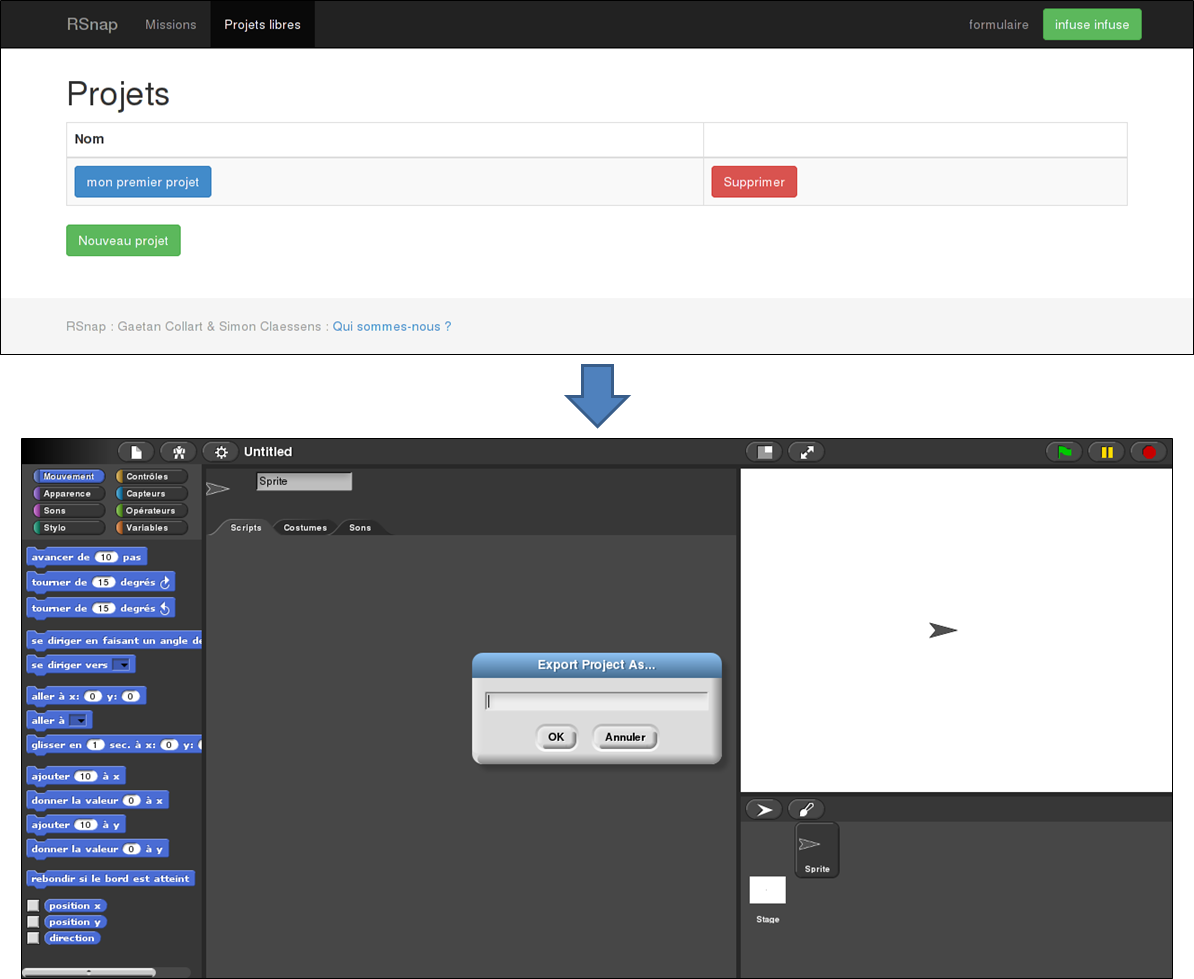
\includegraphics[width=.9\textwidth]{project}
    \caption{Réalisation d'un projet libre}
    \label{fig:project}
  \end{center}
\end{figure}
